This section presents the results of the experiments conducted in this project. The experiments were designed to evaluate the performance of the DSU process in the context of embedded systems, and to investigate the impact of using FRAM as the storage medium for the update process. The main focus of the experiments was to measure the time it takes to perform the update process, and evaluate if the procedure is feasible in a real-time system.

All of the below experiments were conducted on the Texas Instruments MSP430FR5994 microcontroller, running at various clock frequencies. The data was gathered using the built-in debugging tools of the Code Composer Studio IDE. The time estimates were not measured directly but instead calculated based on the number of clock cycles spent in each part of the update process. 

\subsection{Simulated Updates}
As an in depth performance evaluation of the DSU process, a series of simulated updates were conducted. The simulated updates were designed to test the performance of the DSU process under various conditions, such as different update sizes, and using different clock frequencies. The simulated updates were conducted by manually creating \textit{diff} files and applying them to a preallocated array in the upper FRAM of the device. The simulated updates uses only one operation type each, to measure the impact of each operation. In the first series of experiments, the focus is to determine the bottlenecks of the process, as well as how to structure the \textit{diff} files to optimise performance. The second series of experiments focus on the clock frequency of the device, an important factor in deciding the usefulness of FRAM as the storage medium for the device.
\subsubsection{Decode and apply performance}
\subsubsection*{\textbf{\textit{Write operation}}}
Figure \ref{fig:wDecode8} shows the processor cycles required to decode \textbf{Write} operations at different update sizes running at 8MHz. The cycles required to decode the operation is linear with the size of the update, and grows at an increasingly higher rate the more operations are used. As can be seen, this 'context switching' overhead is sizeable, thus effort should be taken to minimize the number of operations required for an update. The maximum update size tested was 256 words for a single operation, and 64 for multiple operations. This is a limitation owing to the small amount of available SRAM on the device. Potential solutions to this limitation are discussed in Section \ref{sec:future_work}. 

\begin{figure}[!ht]
    \centering
    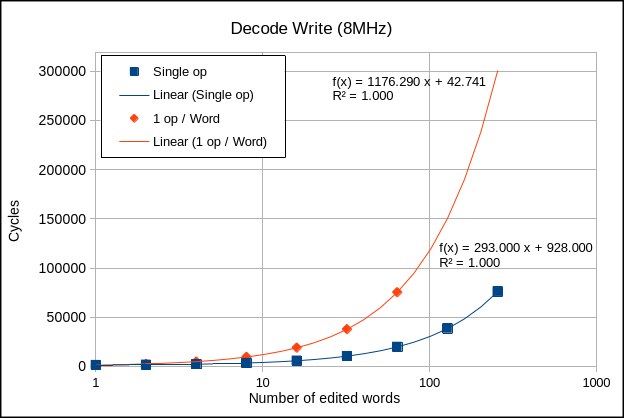
\includegraphics[width=0.9\textwidth]{img/WDecode8.png}
    \caption{Cycles required to decode \textbf{Write} operations running at 8MHz.}
    \label{fig:wDecode8}
\end{figure}
\begin{figure}[!ht]
    \centering
    \includegraphics[width=0.9\textwidth]{img/wApply8.png}
    \caption{Cycles required to apply \textbf{Write} operations running at 8MHz.}
    \label{fig:wApply8}
\end{figure}
Similarly, figure \ref{fig:wApply8} shows the application of the previously discussed updates. The cycles required to apply the updates is also linear with the size of the update, but the rate of growth is lower than that of the decode phase. This is expected since the apply phase only needs to write the data to the specified addresses, while the decode phase needs to read the data from the patch file and translate it into a format that can be applied. This underlines the importance of the decode phase being as efficient as possible, as it is the bottleneck of the DSU process when dealing with \textbf{Write} operations. However, it is also important to note that the apply phase is not negligible. 

\subsubsection*{\textbf{\textit{Shift operation}}}
The opposite, however, is true for the \textbf{Shift} operation, as seen in figure \ref{fig:sDecodeVsApply}. The decode phase runs in constant time with respect to the number of edited words, as there is no need for decoding data. The apply phase, however, grows linearly with the number of words shifted.
\begin{figure}[!ht]
    \centering
    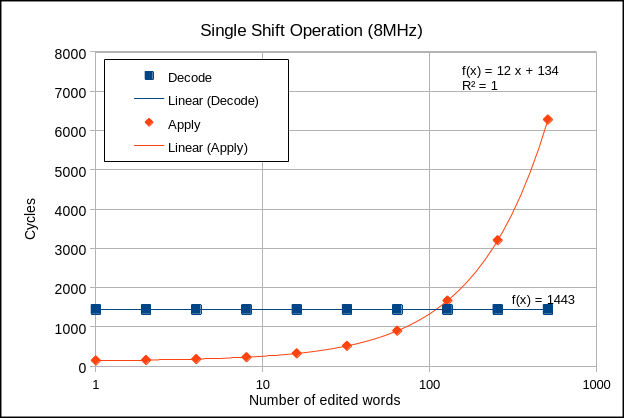
\includegraphics[width=0.9\textwidth]{img/SDecodeVsApply.png}
    \caption{Comparison of Decode and Apply phases for a single \textbf{Shift} operation running at 8MHz.}
    \label{fig:sDecodeVsApply}
\end{figure}

Notably, \textbf{Shift}ing a single word is more expensive than a \textbf{Write} of a single word, but the cost of shifting multiple words is lower than writing multiple words. Thus, the \textbf{Shift} operation should be avoided for single word edits. 

Similarly to the \textbf{Write} operation, effort should be made to minimize the number of \textbf{Shift} operations for any given update, as shown in figure \ref{fig:sDecode8}, where the number of cycles required to decode the operations grows even more rapidly with the number of operations.
\begin{figure}[!ht]
    \centering
    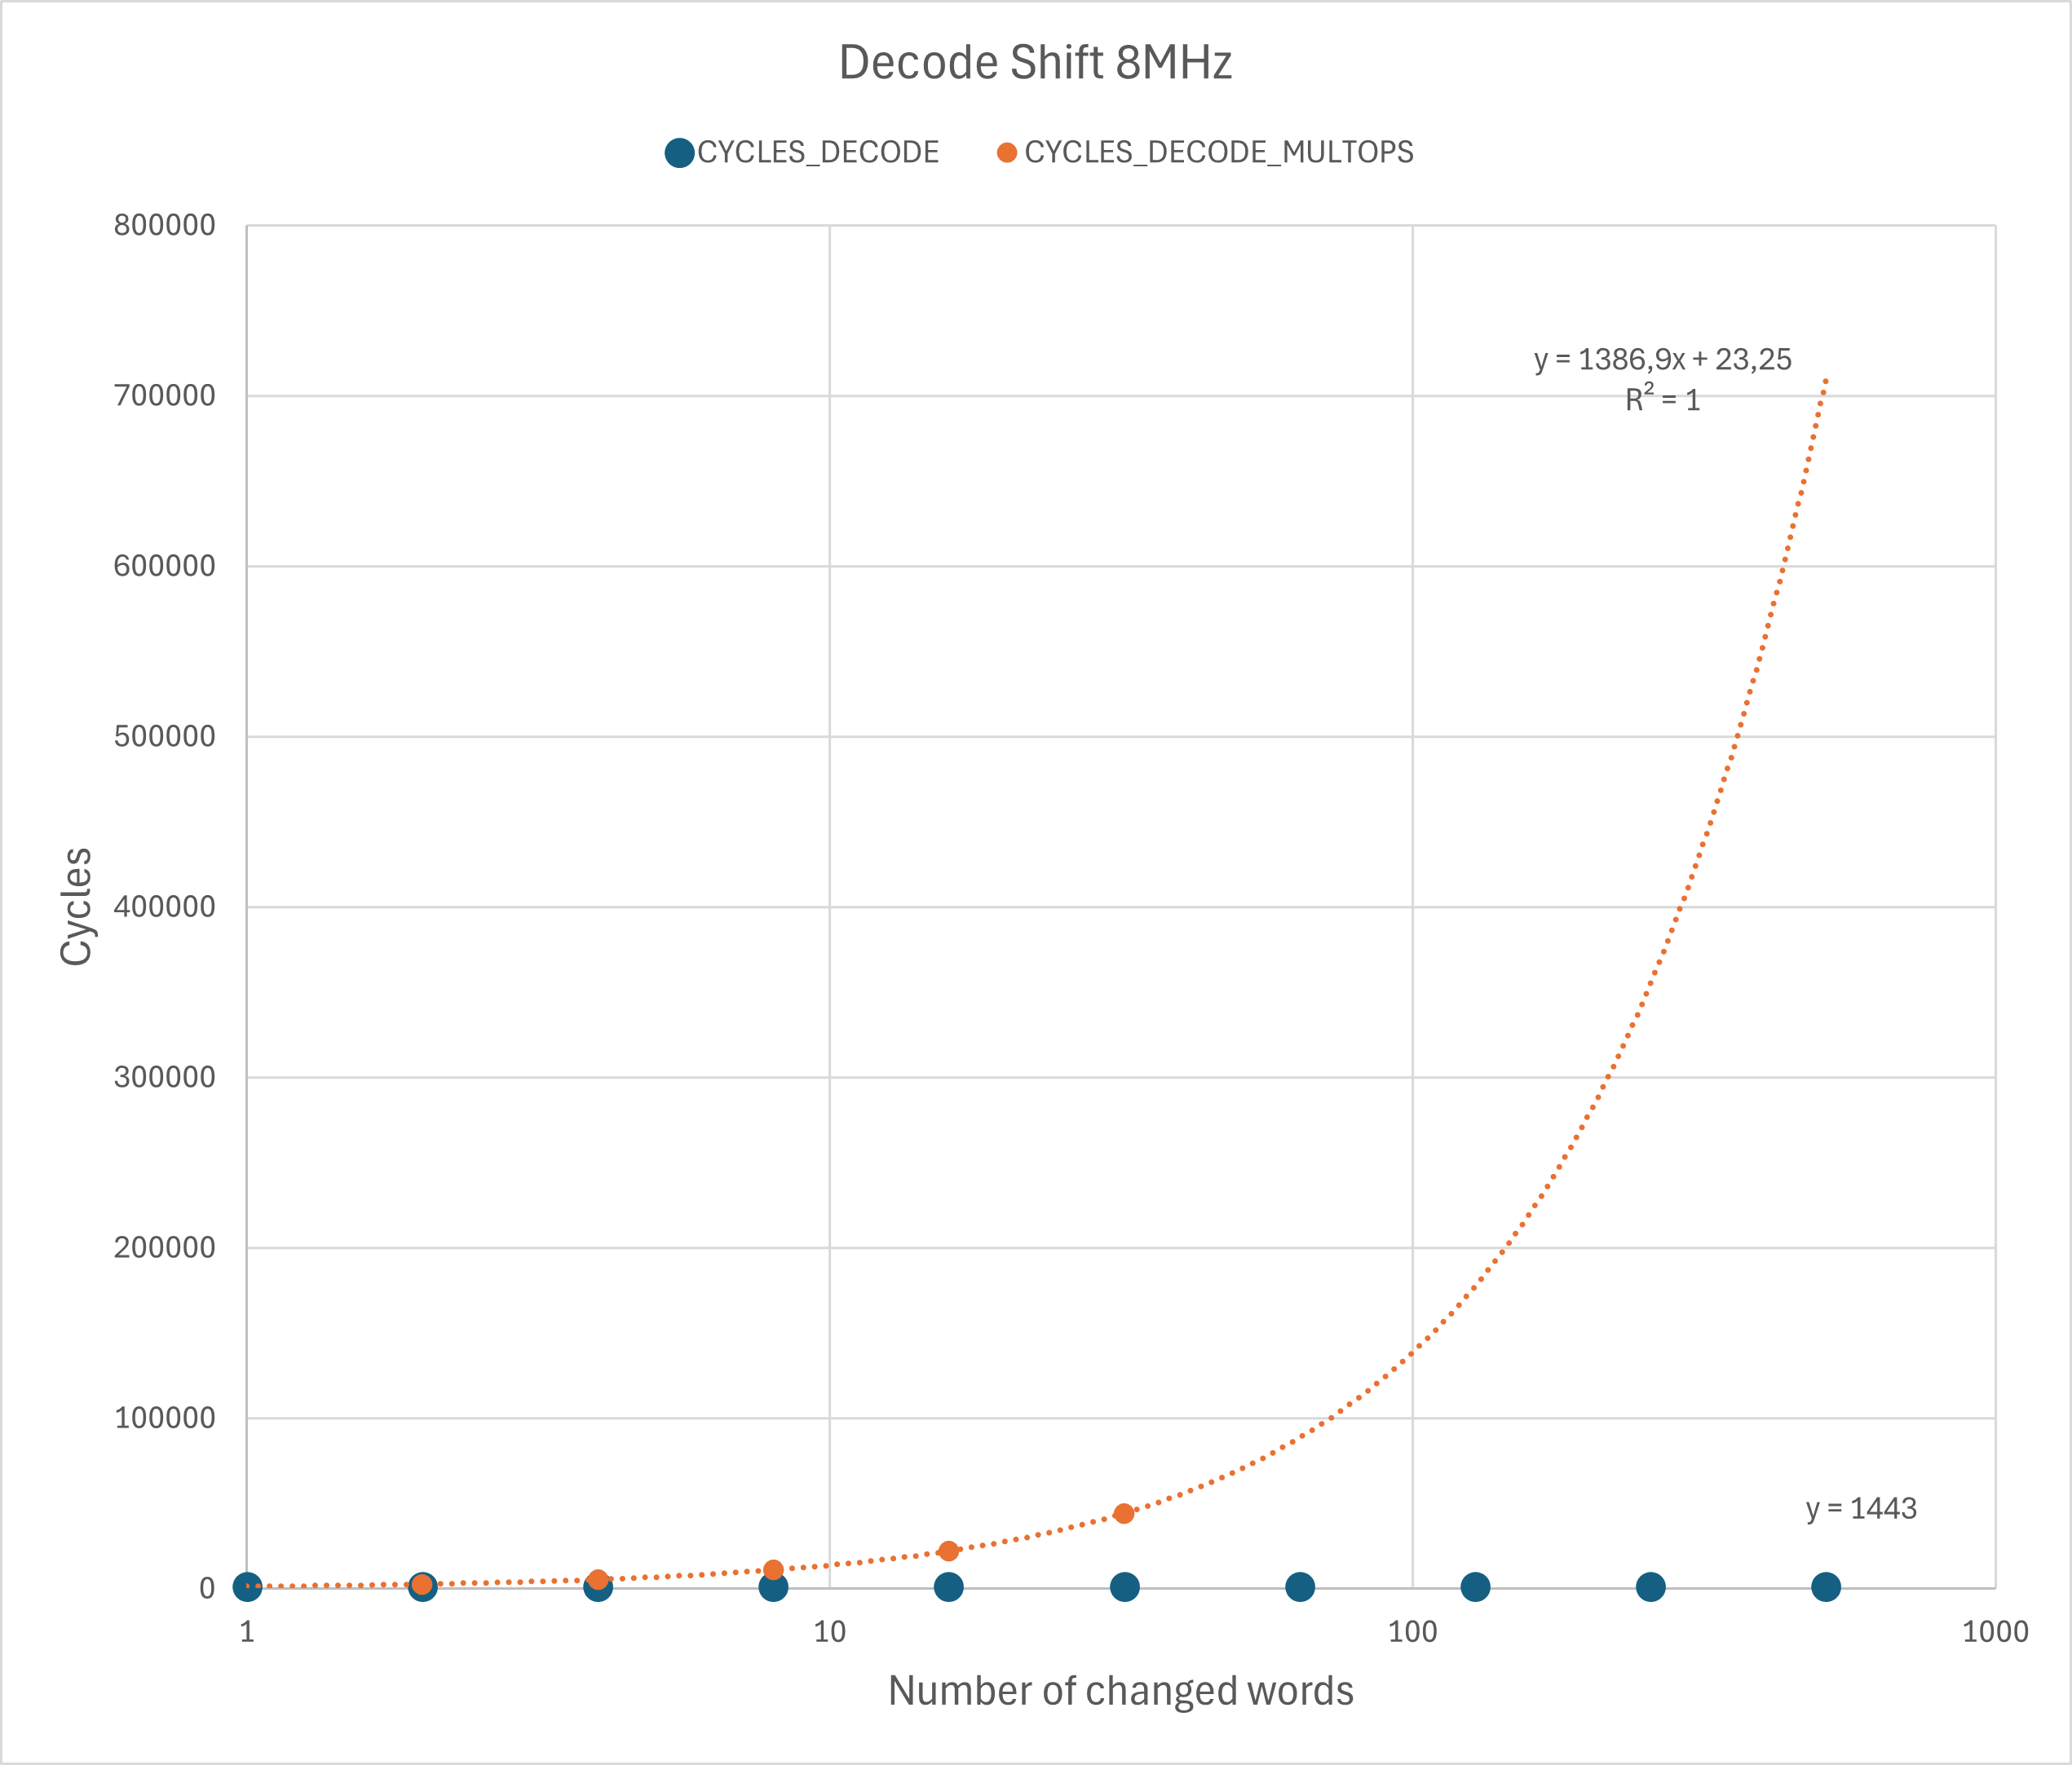
\includegraphics[width=0.9\textwidth]{img/SDecode8.png}
    \caption{Cycles required to decode \textbf{Shift} operations running at 8MHz.}
    \label{fig:sDecode8}
\end{figure}

\subsubsection{Clock frequency impact}
As previously mentioned, the MSP430FR5994 is limited to 8MHz when accessing FRAM. This means running the device at 16MHz will require wait states for every access to FRAM. Although this introduces some overhead in the form of additional cycles required for each access, the overall real-time performance of the update process is should still be improved owing to the faster processing of data.  
In Figure \ref{fig:w8vs16}, the difference in required cycles can be seen when running the same update at different clock frequencies. Even with the added overhead of wait state cycles, the update process is faster at 16MHz than at 8MHz, running at twice the speed but with, on average, $22.9\%$ more cycles required. 
\begin{figure}[!ht]
    \centering
    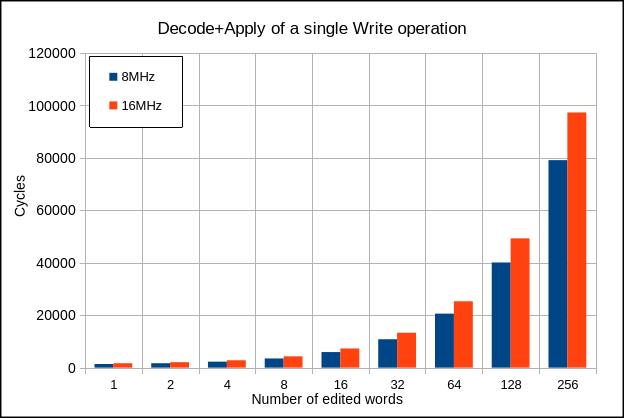
\includegraphics[width=0.9\textwidth]{img/W8vs16.png}
    \caption{Comparison of cycles required to decode and apply \textbf{Write} operations running at 8MHz and 16MHz.}
    \label{fig:w8vs16}
\end{figure}

As Yaacoub et al. show in \cite{NeRTA}, the maximum idle time of a system running Hackflight may be as low as 3ms. Thus, this number is used as a target for the following discussion. Note that this deadline may differ dramatically depending on the application and target system. 

The results of the simulated updates show that the DSU process benefits greatly from a higher clock frequency. 
\begin{figure}[!ht]
    \centering
    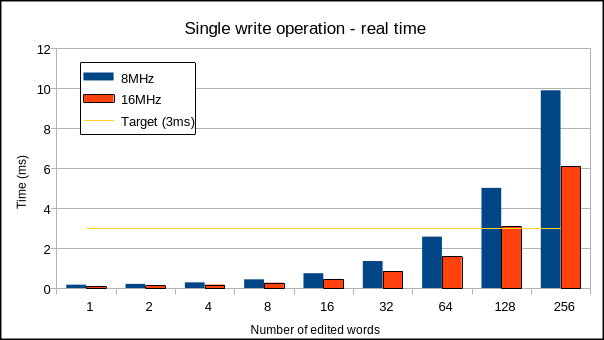
\includegraphics[width=0.9\textwidth]{img/W8vs16_rt.png}
    \caption{Comparison of real time required to decode and apply \textbf{Write} operations running at 8MHz and 16MHz.}
    \label{fig:s8vs16}
\end{figure}

In figure \ref{fig:s8vs16}, the real-time performance of the update process is shown. The real-time performance is calculated by multiplying the number of cycles required to perform the update with the clock cycle time. As can be seen, the real-time performance of the update process is significantly improved when running at 16MHz, with the update process being on average $38.6\%$ faster. This is a significant improvement, and shows that the DSU process is feasible in a real-time system, even with the added overhead of wait states. Furthermore, using a linear regression, an estimated maximum size of a write operation was calculated to 124 words at 16MHz while still meeting the 3ms deadline. At 8MHz, this number is instead 75 words. \todo{shift operation}
\subsection{Proof of Concept Updates}
Firstly, to demonstrate the feasibility of the DSU process, a simple update was constructed which changes a single word in the binary image and makes the LED of the launchpad blink at a different frequency. 
\todo{data}
As expected from such a small update, the time it takes to perform the update is very short, with the majority of time spent in the decoding phase. 

As a more interesting proof-of-concept, a larger update was constructed which changes the behaviour of the LED blinking and introduces new functionality to the application. The application pre-update simply blinks both LEDs on the launchpad at a fixed, synchronized frequency. The post-update application adds functionality to a button on the microcontroller. When pressed changes the blinking frequency of one of the LEDs and makes them unsynchronized, thus providing a more complex update scenario which also has the benefit of being visibly verifiable. 

\noindent\begin{minipage}{.45\textwidth}
\begin{lstlisting}[
    caption={The interrupt service routine before DSU.},
    label={lst:pre_dsu_isr}
]
if (P5IFG & BIT5)
{ // Button 1 pressed
    update(diff);
}

P5IFG &= 0; // Clear interrupt flag
\end{lstlisting}
\end{minipage}\hfill
\noindent\begin{minipage}{.45\textwidth}
\begin{lstlisting}[
    caption={The interrupt service routine after DSU.},
    label={lst:post_dsu_isr}
]
if (P5IFG & BIT5)
{ // Button 1 pressed
    update(diff);
} 
if (P5IFG & BIT6)
{ // Button 2 pressed
    green_period += 1000;
}

P5IFG &= 0; // Clear interrupt flags
\end{lstlisting}
\end{minipage}\hfill
The update took a total of 6151 cycles to complete at 8MHz, with the majority of the time spent in the decode phase. The update process was completed in 0.76ms, which is well within the 3ms deadline. While this proof-of-concept is still relatively simple, requiring only a single \textbf{Shift}- and \textbf{Write} operation each, it demonstrates the potential of the DSU process. 
